V této kapitole si popíšeme jak dron ovládat a zdali opravdu funguje.

\section{Připojení se}
    Po zapojení baterie se dron automaticky zapne. Několik vteřin na to se vytvoří Wi-Fi access point, který se základně jmenuje "Drone" a lze se k němu připojit za pomocí hesla "password". Jak jméno, tak heslo pro AP se dá změnit v kódu přepsáním proměnných *ssid a *password. Návod na nahrání upraveného kódu se podívejte do kapitoly 4.3. Pokud dron chcete ovládat, je zapotřebí se na tento AP připojit. Veškeré ovládání poté najdete ve vašem webovém prohlížeci na  adrese "192.168.4.1". K ovládání doporučuji používat mobilního telefonu, ale je možné využít i počítače.

\section{Ovládání}
    Na webové stránce vidíte jednoduché GUI, s devíti tlačítky - osm na samotné ovládání drona a jedno na updatování firmware. Pro zapnutí motorů drona zmáčkněte tlačítko "ON". Dále pro vzlédnutí využijte levého dolního tlačítka "UP" a pro pokles tlačítka "DOWN". Pro pohyb do stran využijte čtyři tlačítka určena pro každý ze čtyř základních směrů.
    
\vspace{5mm}

    \begin{figure}[h]
        \centering
        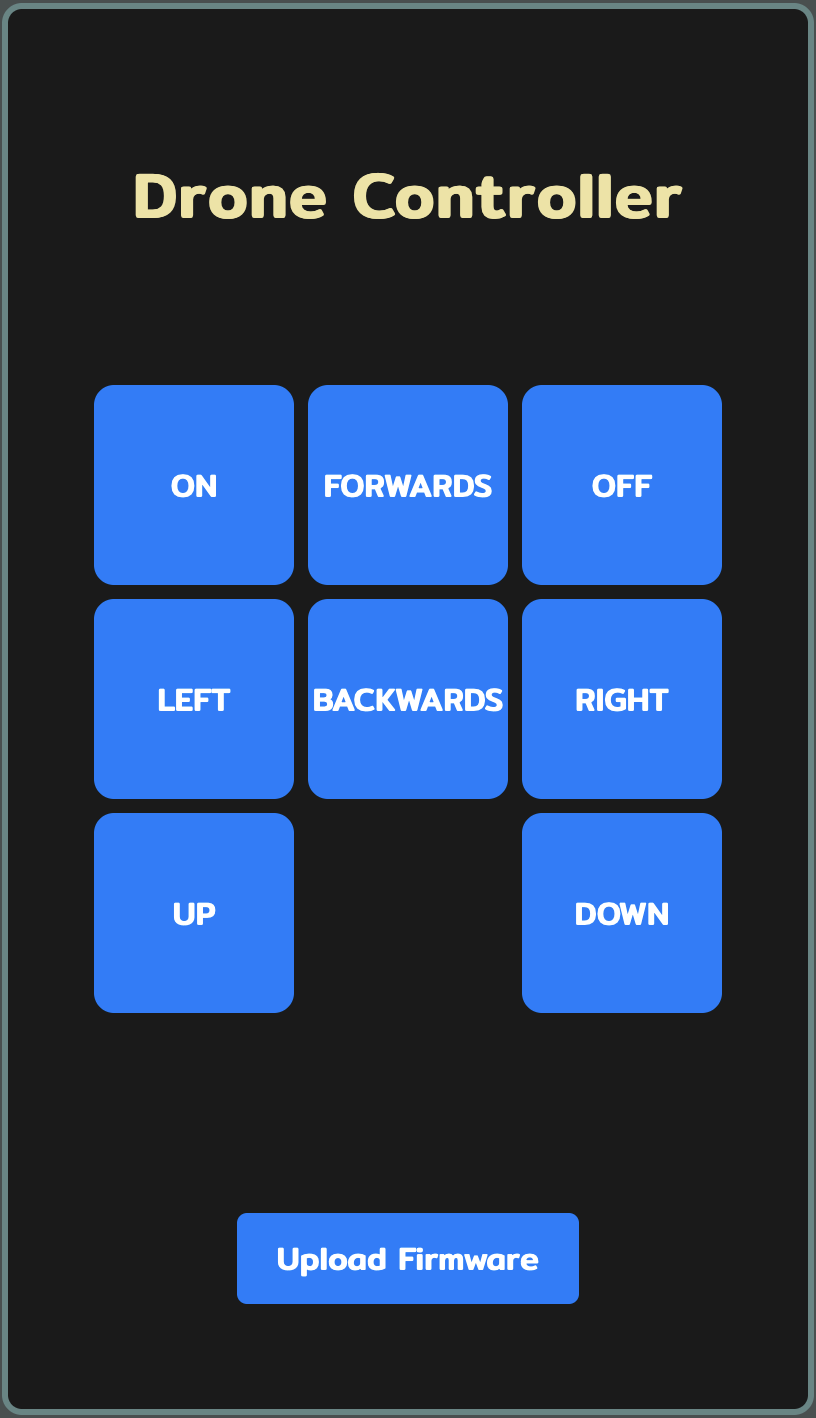
\includegraphics[scale=0.4]{img/gui.png}
        \caption{Webové rozhraní}
    \end{figure}

\newpage
    
\section{Updatování}
    Změnu firmware provádějte pouza na vlastní nebezpečí. Přepsání jakékoliv části základního kódu může způsobit nefunkčnost drona. Pokud jste se rozhodli si kód jakkoliv upravit, můžete ho jednoduše nahrát přes webové rozhraní. Pokud se nacházíte na ovládacím panelu popsaném v předchozí části, zmáčkněte dolní tlačítka "Upload Firmware". Toto vás přesměruje do updatovacího rozharní. Zaškrtněte políčko "Firmware" a vyberte binárku s vaším kódem. Během procesu flashování NEODPOJUJTE dron od baterie.

\section{Skutečné použití}
     I přes veškerou snahu se dron není schopen sám zvednout. Je tomu tak z důvodu příliš vysoké hmotnosti drona, ze kterého motory nemají dostatečný tah pro vzlet. Více než polovina hmotnosti je tvořena samotnou baterií. Dále by bylo dobré zvážit použití jiných vrtulí. Všechny ostatní funkce fungují. Jediné co by na dronu s nižší hmotností bylo potřeba doladit jsou konstanty u vyvažování pomocí gyroskopu a základní rychlost motorů, kterou se otáčejí bez zadaných příkazů.